\documentclass{amsart}

\usepackage{graphicx, fancyhdr, rotating, float} % see geometry.pdf on how to lay out the page. There's lots.
\usepackage[a4paper, margin=0.5in, includeheadfoot, headheight=2cm, footskip=2cm]{geometry}
\usepackage{booktabs}
\usepackage{multirow}


\usepackage{color}
\usepackage{xcolor}
\usepackage{listings}
\usepackage{numprint}
\npthousandsep{,}

\usepackage{caption}
\DeclareCaptionFont{white}{\color{white}}
\DeclareCaptionFormat{listing}{\colorbox{gray}{\parbox{\textwidth}{#1#2#3}}}
\captionsetup[lstlisting]{format=listing,labelfont=white,textfont=white}



% See the ``Article customise'' template for come common customisations
\providecommand{\e}[1]{\ensuremath{\times 10^{#1}}}
%\setlength{\headheight}{2cm}

\graphicspath{{./images/}} % Specify images directory


% Title and document details
\newcommand{\titleinfo}{$job.title} 
\title{\titleinfo}
\pagestyle{fancy}
\fancyhf{}
\lhead{}
\chead{
\includegraphics[height=2.5cm]{header.png}}
\renewcommand{\headrulewidth}{0pt}
\rhead{}
\rfoot{\thepage}
\lfoot{\titleinfo}
\author{$job.author}
\date{}

%%% BEGIN DOCUMENT
\begin{document}

% First page (title and toc)
\maketitle
\thispagestyle{fancy}
\tableofcontents


% General spacing for the document to use after the title and toc
\linespread{1.2} % A little more line spacing than usual
\setlength\parindent{0pt} % Removes indentation from paragraphs
\setlength{\parskip}{0.25cm} % Adds an extra bit of linespacing between paragraphs
\setlength{\belowbottomsep}{2ex} % Ensure a decent gap before the footer



\newpage
\section{General Information}
\begin{description}
\item[Project title] \titleinfo
\item[Name of collaborator] $job.collaborator
\item[Staff member] $job.author
\item[Master JIRA ticket] xxx
\item[SEQINFO ticket] $job.jiraSeqinfoId
\item[SEQOP ticket] xxx
\item[MISO ticket] $job.misoId
\item[Sequencing instrument] xxx
\item[Start date of analysis] xxx
\item[End date of analysis] \today
\end{description}


\section{Software Used}

This first pass assembly was built with RAMPART (Robust AutoMatic first Pass Assembly Toolkit).  RAMPART is an open source project created by TGAC.  It makes use of a number of other tools in its pipeline:

\begin{description}

\item[Abyss-1.3.4] A modified version of Abyss that handles large k-mer sizes (up to 127) to do the sequence assembly
\item[SSPACE-BASIC-2.0] To build enhance scaffolds
\item[GapCloser-1.12] To close gaps in the scaffolds
\item[R-2.15.0] To produce graphs and analyse assembly statistics
\item[Exonerate-2.2.0] To identify PhiX scaffolds
\end{description}



\newpage
\section{Quality Trimming}

Raw:

#foreach($lib in $job.libsRaw)

Library Name: $lib.name
Max Read Length: $lib.readLength
Average Insert size: $lib.averageInsertSize


#end

The raw reads were analysed based on the sequence quality scores, and those sequences which dipped below a certain threshold were either trimmed or excluded.  The tools Sickle v1.1 was used to do this.  This tool was configured so that the 3' ends of reads are trimmed where quality degrades beyond a threshold score of Q-rgqtscore.  Any trimmed reads must still exceed the -rgqtminlen base pairs in length otherwise the whole read is discarded.


\subsection{Dataset Statistics}

Table \ref{tab:dataset-stats} shows some basic properties for each dataset.

\begin{table}[h]
\begin{tabular}{lllrrrr}
\toprule
Library & Dataset & File & Total Unpaired Reads & \%GC & Total Bases & Estimated Coverage  \\ \midrule
#foreach($lib in $job.libsRaw)
$lib.name & $lib.dataset & PE1 & \numprint{$lib.filePaired1.seqCount} & $lib.filePaired1.gCContent & \numprint{$lib.filePaired1.baseCount} & $0 \times$ \\ 
$lib.name & $lib.dataset & PE2 & \numprint{$lib.filePaired2.seqCount} & $lib.filePaired2.gCContent & \numprint{$lib.filePaired2.baseCount} & $0 \times$ \\
#if( $lib.seFile )
$lib.name & $lib.dataset & SE & \numprint{$lib.seFile.seqCount} & $lib.seFile.gCContent & \numprint{$lib.seFile.baseCount} & $ xxx \times$ \\
#end
#end
#foreach($lib in $job.libsQt)
$lib.name & $lib.dataset & PE1 & \numprint{$lib.filePaired1.seqCount} & $lib.filePaired1.gCContent & \numprint{$lib.filePaired1.baseCount} & $0 \times$ \\ 
$lib.name & $lib.dataset & PE2 & \numprint{$lib.filePaired2.seqCount} & $lib.filePaired2.gCContent & \numprint{$lib.filePaired2.baseCount} & $0 \times$ \\
#if( $lib.seFile )
$lib.name & $lib.dataset & SE & \numprint{$lib.seFile.seqCount} & $lib.seFile.gCContent & \numprint{$lib.seFile.baseCount} & $ xxx \times$ \\
#end
#end

\bottomrule
\end{tabular}
\caption{Basic Statistics for each dataset.  Estimated Coverage assumes even distribution of reads against a genome size of 5.9Mb.}
\label{tab:dataset-stats}
\end{table}



\pagebreak
\newpage
\section{Diagrammatic Representation of the Complete Workflow}

Figure \ref{fig:workflow} represents the general workflow applied to the raw reads produced from the sequencing device.  Initially multiple datasets are produced, then each of these is processed through an assembler using multiple k-mer values producing multiple assemblies.  These assemblies are analysed and the best assembly is selected to be enhanced using multiple iterations of SSPACE and GapCloser.  The resulting file has scaffolds under 1KB removed before a final screening process is applied.

\begin{figure}[H]
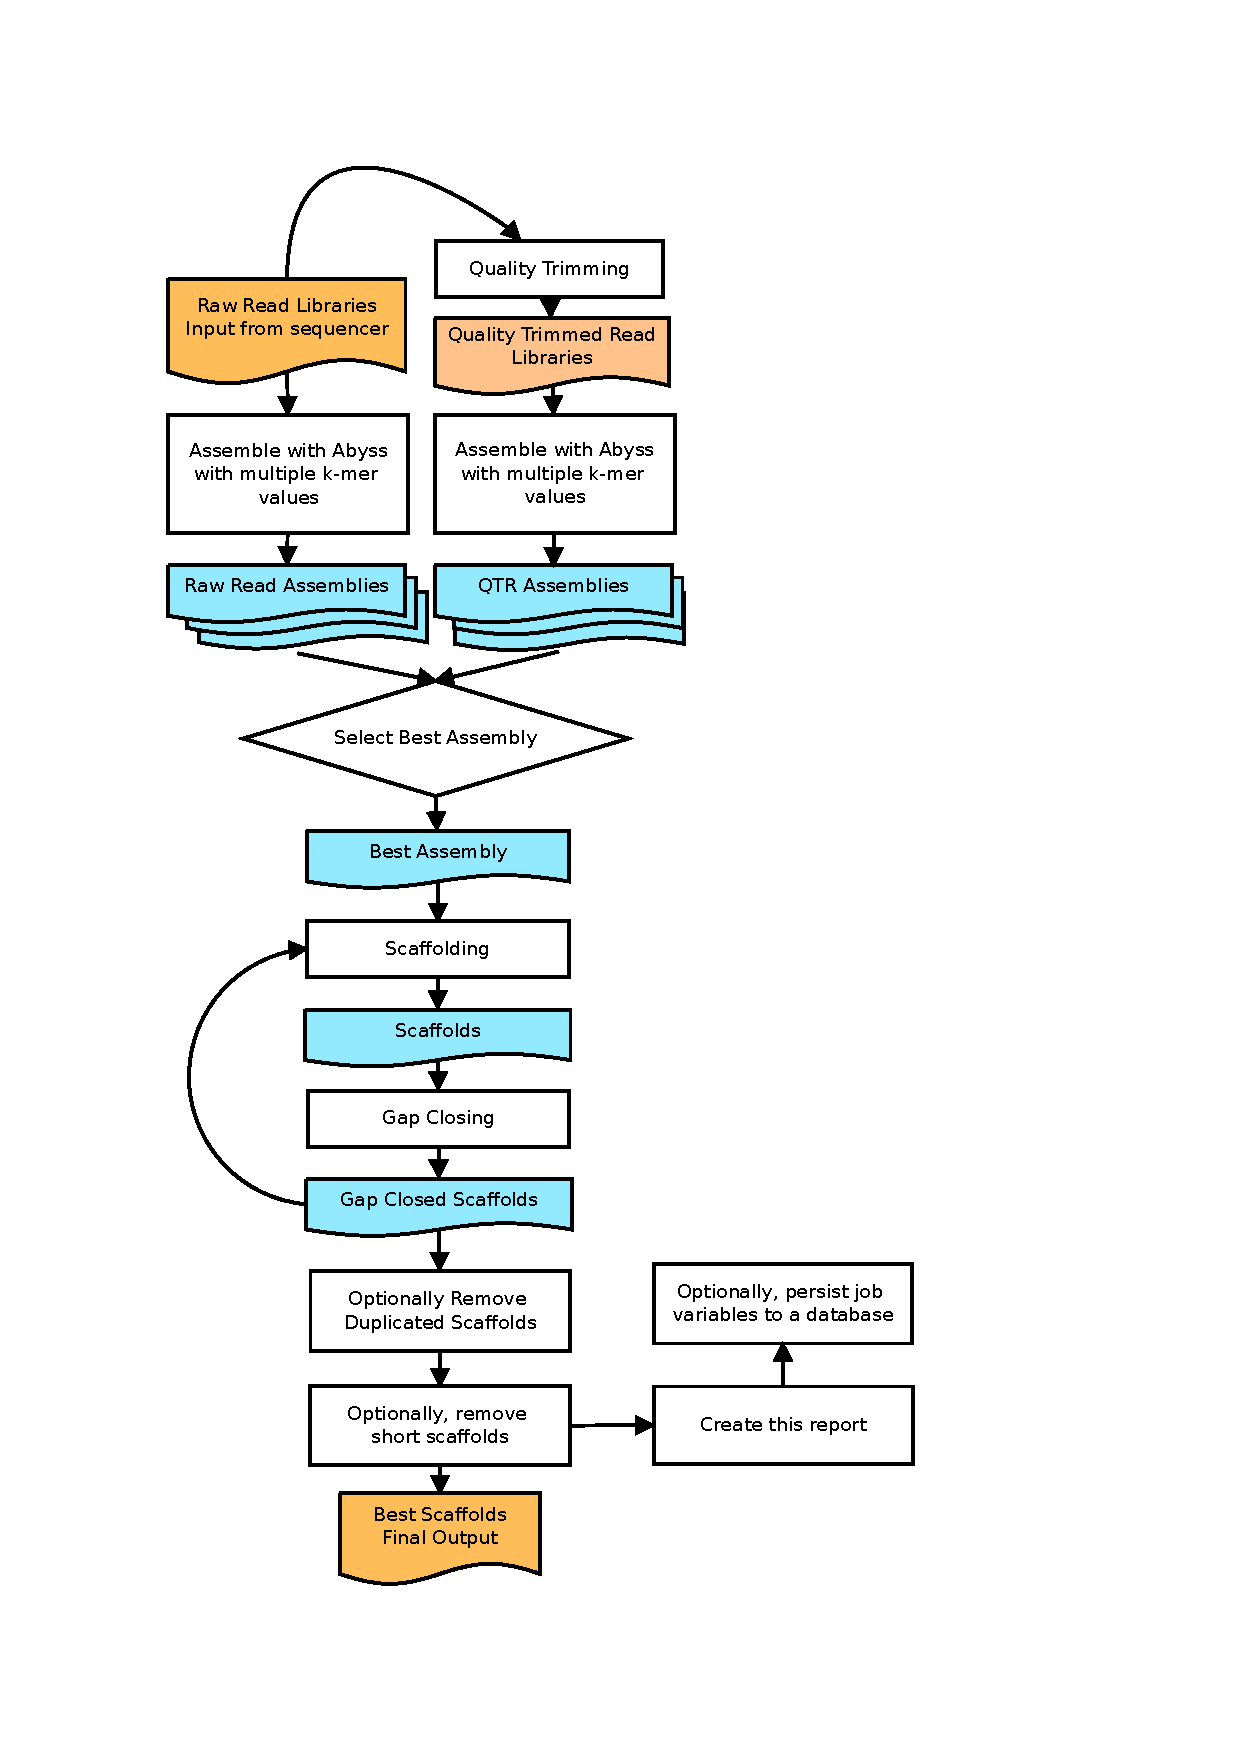
\includegraphics[width=13cm]{Workflow.pdf}
\caption{Typical First Pass Assembly Workflow}
\label{fig:workflow}
\end{figure}



\newpage
\section{Assembly Workflow}

The datasets we assembled the reads into using a variety of k-mer lengths to determine the optimal k-mer setting from which to build the final assembly. 

\begin{table}[H]
\begin{center}
\begin{tabular}{c|c|c}
\includegraphics[height=5cm]{Mass_NBC.pdf} & \includegraphics[height=5cm]{Mass_TB.pdf} & \includegraphics[height=5cm]{Mass_N.pdf}\\ \midrule 
\includegraphics[height=5cm]{Mass_AL.pdf} & \includegraphics[height=5cm]{Mass_ML.pdf} & \includegraphics[height=5cm]{Mass_N50.pdf} 
\end{tabular}
\end{center}
\caption{Plots describing Assembly Quality Metrics vs kmer value. Black lines represent the Raw Dataset, blue lines the quality trimmed dataset and red lines represent the contaminant screened dataset. }
\label{fig:aq_b}
\end{table}

RAMPART's interpretation of the assembly results suggests that using a k-mer value of $best_mass_asm.kmer on from the $best_mass_asm.dataset dataset generates the best scaffolds.  For a description of how RAMPART selects the best scaffold consult the RAMPART documentation.  The assembly statistics are shown in table \ref{tab:scaffold-stats}. 

The scaffolds for the chosen assembly was then enhanced using the with SSPACE and GapCloser run over -rgimpiterations iterations.  The results of this step are shown in the Table \ref{tab:scaffold-stats}.

Deduplication

Clipping



\begin{table}[H]
\begin{tabular}{lrrrrr}
\toprule
Dataset & Number of Scaffolds & Total Bases & Average Length & Maximum Length & N50 \\
\midrule
%Abyss Raw K121 	& 281 & 6249378 & 22239 & 429067 & 167654 \\
%SSPACE 1    		& 268 & 6257399 & 23348 & 466346 & 170809 \\
%GapCloser 1		& 268 & 6257401 & 23348 & 466347 & 170809 \\
%SSPACE 2    		& 267 & 6257418 & 23436 & 466347 & 170809 \\
%GapCloser 2		& 267 & 6257419 & 23436 & 466347 & 170809 \\
%SSPACE 3    		& 267 & 6257419 & 23436 & 466347 & 170809 \\
%GapCloser 3		& 267 & 6257420 & 23436 & 466347 & 170809 \\
%PhiX removed (Final) 	& 266 & 6251260 & 23436 & 466347 & 170809 \\
%Clipped (Final)			& 137 & 6217122 & 45096 & 466347 & 170809 \\
\bottomrule
\end{tabular}
\caption{Assemblies progressively improved via scaffolding, gap filling, screening and clipping steps, starting from the raw k121 assembly.  }
\label{tab:scaffold-stats}
\end{table}


\newpage
\section{Accessing the Data}


The original reads, as well as the contaminant screened and quality trimmed reads can be found at the following location:

\begin{lstlisting}[label=path:1]
\end{lstlisting}

\emph{Note}: The contaminant screened reads and assemblies referred to in this report can be identified by the *.screened2.* tag.  The quality trimmed reads referred to in this report can be identified with the *.sickle.* or *.trimmed.* tag.

The Abyss assemblies and statistics for each dataset can be found at the following location:

\begin{lstlisting}[label=path:1]
$mass_dir
\end{lstlisting}


The assemblies, statistics and other data for the assembly improvement stage can be found at the following location:

\begin{lstlisting}[label=path:1]
$improver_dir
\end{lstlisting} 


Two final assemblies are provided, one with the complete set of scaffolds, on with on those 1Kb and above.  These assemblies can be found at the following locations:

\begin{lstlisting}[label=path:1]
$final_asm.filePath
\end{lstlisting}


\end{document}
